 \chapter{Implementation and Testing}

This chapter will discuss the implementation and testing of both parts of the project. This chapter does not include all implementation details, instead it focuses on the more important and challenging aspects of the project. For more details about the exact implementation, a reading of the source code is recommended.

\section{Library: connecting to a MySQL server and executing queries} \label{ch:impllib:sec:connecting}
To connect to a MySQL server, the library uses the Ruby library mysql2. The library, or gem as it is called in Ruby, provides the implementation for connecting, querying and retrieving results from a MySQL server. mysql2 is binding to MySQL's C library libmysql. mysql2 is the more modern and lean version of the mysql gem. According to the project's Github page, mysql2 can be two times faster than mysql. Furthermore, mysql2 is also much more popular with over 42 million downloads on RubyGems, compared to mysql's 8 million downloads.

To connect to a MySQL server, the library requires the address and port of the server, and an account and password. The account must be the root user or at least one that has the permission to create and drop databases, to create and drop users, and to grant permissions to an user.

\subsection{Handling concurrent submissions}

As the library will be used in a web application, concurrency cannot be avoided. Users can submit solutions at any time and it is possible that two users submit solutions at the same time. Obviously, concurrency can be ignored by limiting the execution of only one compile or assessment at a time. However, this solution can lead to frustrating waiting times and requires the implementation of background workers to perform the work. Therefore, the tool opted to implement a solution that allows concurrent executions.

To allow concurrency, each submission or compilation is performed using different connections to different databases (a MySQL server can have multiple databases). Every compilation or submission begins by creating a new and unique database based on the current time. The database name will follow the format \texttt{HOURMINUTESECOND}. While this should cover most cases, due to the concurrent nature of the application, it might be the case that two connections try to create a database with the same name. However, MySQL ensures that if two create database statements with the same database name are executed at the same time, at least one create will fail. In this case, we repeat all failed creations (by using the new time) until they succeed. On second and further attempts, we also add a \mintinline{ruby}{_attempt} at the end of the database name to reduce the chance of another conflict. At the end of the compilation, the newly created database will be dropped.

%TC:ignore
\begin{code}
    \begin{minted}{ruby}
success = false
attempt = 0
while !success do
  time = DateTime.now

  if attempt > 0
    @database = "#{Time.now.strftime("%H%M%S")}_#{attempt}"
  else
    @database = "#{Time.now.strftime("%H%M%S")}"
  end

  begin
    @client.query("CREATE DATABASE `#{@database}`")
    success = true
  rescue Mysql2::Error => exception
    raise exception unless exception.message.include?("database exists")
    success = false
    attempt += 1
  end
end
\end{minted}
    \caption{Creating a new database for each run}
    \label{fig:creating_new_database}
\end{code}
%TC:endignore

\subsection{Preventing malicious actions from input SQL queries}

Considering that the library executes arbitrary queries, the risks associated with malicious SQL are significant. The application never returns back the query results which means the potential for data leaking by abusing the execution of arbitrary queries does not exist. However, an arbitrary query can destroy or modify other databases on the MySQL server. Therefore, the library must take extra precautions as it deals with unchecked user code. To prevent malicious actions, we created a new MySQL user that only has permission for the newly created database.

%TC:ignore
\begin{code}
\begin{minted}{ruby}
@client.query("CREATE USER IF NOT EXISTS `#{@database}`;")
@client.query("GRANT ALL PRIVILEGES ON `#{@database}`.* TO `#{@database}` WITH GRANT OPTION;")
\end{minted}
\caption{Creating a new user with permissions for the new database}
\label{fig:creating_new_user}
\end{code}
%TC:endignore

All queries are performed using this MySQL user, instead of using the root one. The temporary user is deleted at the end of the compile / assessment execution. This way, the user input can only damage the created database for his assessment. However, this is not an issue considering these are short-lived databases which are destroyed at the end of the assessment.

The only way to get around the limitation of the restricted user would be to use a different user. Changing the user in MySQL is not possible through a SQL command. The only possible way would be to use the \texttt{system} command which executes bash code in combination with the \texttt{mysql -uroot --password} bash command if they knew the root password, but not the url of the database. However, the \texttt{system} command is only available on connections opened with the \texttt{mysql} bash command, which is not the case for \texttt{mysql2} - so users cannot exploit this method. Furthermore, the user has limited permissions so they cannot run commands such as \mintinline{mysql}{SET PASSWORD} to change existing users.

\section{Library: parsing and transforming queries}

During the canonicalization and grading process, SQL queries will go through multiple transformations after being parsed and separated in independent components. MySQL does not provide an official parser for any programming language, so the library had to use a 3rd party tool. The advantage of using an existing parser is that we can ignore the implementation details of parsing.

The library initially used the sql-parser Ruby gem. Throughout the development process, there have been multiple problems associated with this tool. Most importantly, the library did not have support for multiple SQL statements we required. Unfortunately, many issues with sql-parser were discovered only late in the project.

An alternative was represented by the pg\_query Ruby gem. Internally, it uses PostgreSQL's parsing library libpg\_query built in C++. pg\_query provides much better code and stability, due to its nature of being part of a production database system, compared to sql-parser which is only used for parsing. PostgreSQL, like MySQL, is a widely used database system, being the 4th most used database engine according to \cite{db_engine:statistics}. Although both PostgreSQL and MySQL have SQL at their core, each one implements their own version of SQL. Therefore, a query might work in MySQL, but not work in PostgreSQL, or return different results. For instance, in MySQL string comparison is case insensitive, while in PostgreSQL it is not. In addition, each SQL version adds their own functions that diverge from Standard SQL. Therefore, implementing pg\_query turned out to be impossible due to the many differences in syntax between the two SQL versions. In addition, time constraints made it unjustifiable to spend time on re-implementing all transformers already built.

\subsection{Extending sql-parser}

In the end, due to the issues described previously, a decision was made to continue using sql-parser. Fortunately, sql-parser uses an MIT license which allowed us to fork the library and implement the fixes in the fork. The parser was implemented using Racc's grammar files. According to the GitHub page of the tool, Racc is a \textit{LALR(1) - "Look Ahead Left to Right" -  parser generator} that generates Ruby code. The fork created implemented the following functionality:
\begin{itemize}
    \item Support for \mintinline{mysql}{DISTINCT}, \mintinline{mysql}{DISTINCTROW}, \mintinline{mysql}{ALL} in \mintinline{mysql}{SELECT} statements
    \item Support for \mintinline{mysql}{LIMIT} and \mintinline{mysql}{OFFSET}
    \item Support for using a qualified column in \mintinline{mysql}{ORDER BY} clause
    \item Support for using the columns number in \mintinline{mysql}{GROUP} clause
    \item Support for using sub-queries in \mintinline{mysql}{FROM} clause
    \item Fix problems with two strings being considered just one string
    \item Support for \texttt{\%} operation
    \item Support for arithemtic operations in \mintinline{mysql}{FROM}, \mintinline{mysql}{Order}
    \item Support for \texttt{;} at the end of a query
\end{itemize}

The process of adding a new feature was the following:
\begin{enumerate}
    \item Create a \mintinline{ruby}{Node} class representing the new clause, if a new clause was implemented. A \mintinline{ruby}{Node} represents an element of a query: a clause, a number, a word, a condition, etc. For instance, the newly created \texttt{LIMIT} node has the following structure:
\begin{code}
\begin{minted}{ruby}
class LimitClause < Node
    def initialize(limit, offset)
        @limit = limit
        @offset = offset
    end

    attr_reader :limit, :offset
end
\end{minted}
\caption{Limit clause \mintinline{ruby}{Node}}
\label{fig:limit_clause}
\end{code}
    \item Update any existing \mintinline{ruby}{Node}s to link to the newly created node. For instance, the \mintinline{ruby}{LimitClause} node had to be linked to the \mintinline{ruby}{TableExpression} node.
    \item Add the new parsing rules to Racc grammar file. For instance, when adding the LIMIT clause there are three options: there is only a limit number, there are two numbers for limit and offset separated by the word \texttt{OFFSET}, or the two numbers are separated by a comma:
    
\begin{code}
    \centering
    \begin{minted}{ruby}
  limit_clause
: # no action
| LIMIT unsigned_integer { result = SQLParser::Statement::LimitClause.new(val[1], nil) }
| LIMIT unsigned_integer OFFSET unsigned_integer { result = SQLParser::Statement::LimitClause.new(val[1], val[3]) }
| LIMIT unsigned_integer comma unsigned_integer { result = SQLParser::Statement::LimitClause.new(val[3], val[1]) }
    \end{minted}
    \caption{Limit clause \texttt{Racc}}
    \label{fig:limit_clause_racc}
\end{code}
\end{enumerate}

\subsection{Using sql-parser to parse SQL queries}
Using sql-parser to parse SQL queries is straightforward. The library provides the \mintinline{mysql}{scan_str} which transforms a string (the SQL query) into a SQL Abstract Syntax Tree (AST). The AST is formed of multiple nodes. As mentioned in the last section, a node is a component of the clause. The general structure of the AST for a SELECT query is presented in figure \ref{fig:select_ast}.

\begin{figure}[ht]
\centering
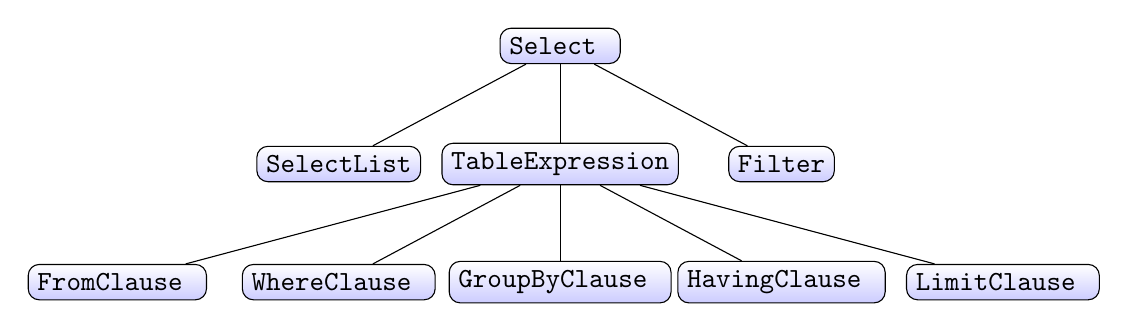
\begin{tikzpicture}[sibling distance=8em,
  every node/.style = {shape=rectangle, rounded corners,
    draw, align=center,
    top color=white, bottom color=blue!20}]]
  \node { \ttfamily Select }
    child { node {\ttfamily SelectList} }
    child { node {\ttfamily TableExpression}
        child { node {\ttfamily FromClause } }
        child { node {\ttfamily WhereClause } }
        child { node {\ttfamily GroupByClause } }
        child { node {\ttfamily HavingClause } }
        child { node {\ttfamily LimitClause } } }
    child { node {\ttfamily Filter} };
\end{tikzpicture}
\caption{General structure of the SELECT's AST}
\label{fig:select_ast}
\end{figure}
All the leaves presented in figure \ref{fig:select_ast} also have their nodes. For instance, SelectList has an array of columns which can be of many types (QualifiedColumn, Column, AggregateColumn, etc.). In addition, what we previously called Boolean components (WHERE and HAVING) have both subtrees representing the Boolean expression.


\subsection{Using sql-parser to change queries}
sql-parser also provides a way to change a parsed query (which is now a combination of multiple Nodes) back to a SQL query. Unfortunately, the process of internally modifying the structure of a query is not well-defined and there is no public interface exposed. Each node has one or more private instance variables that represent the values of the Node. For instance, the limit node shown in listing \ref{fig:limit_clause}, has two such variables: limit and offset. sql-parser does not provide a way to change these properties as all Nodes expose just a reader method (set using \mintinline{ruby}{attr_reader}). Fortunately, Ruby provides a \mintinline{ruby}{instance_variable_set} method which allows anyone with a reference to an object to change that object's internal variables even if they are private and no setter is exposed. It is worth mentioning that, while this approach might work, the use of \mintinline{ruby}{instance_variable_set} goes against the principle of encapsulation, and might mean that a future update to the library can lead to errors, if the internal structure of Nodes is modified.
\begin{code}
\begin{minted}{ruby}
@parsed_query.query_expression.list.instance_variable_set(
  "@columns",
  new_columns
)
\end{minted}
\caption{Example of updating the column list for a parsed query}
\end{code}

After a query is modified, sql-parser exposes a \mintinline{ruby}{.to_sql} method on each Node that can be used to transform a Node to a SQL statement.

\section{Library: handling sub-queries}

Unfortunately, compared to XData, the library cannot handle submissions that include sub-queries. Some work to implement this has been attempted and is available in the current code: canonicalization of sub-queries, comparison of nested queries, updating sql-parser to support sub-queries in the FROM clause, etc. Unfortunately, this has been added very late in the project meaning that most existing work had to be redone for supporting sub-queries which, due to time constraints, was not possible. That is because some parts of the library made the assumption that no sub-queries are present.

\section{Library: canonicalizing queries}

As previously mentioned in section \ref{ch:lit:sec:improved_canon}, the library will implement a canonicalization step. The library implements all canonicalizations done by XData described in section \ref{ch:lit:sec:canonicalization}, and the additional ones presented in section \ref{ch:lit:sec:improved_canon}. All transformations use sql-parser's transformations ability combined with the ability to make queries on the database.

As mentioned in the design section \ref{ch:lit:sec:improved_canon}, the canonicalization process is done sequentially in a specific order that ensures later canonicalizations do not make changes that are incompatible with previously executed transformations. 

\begin{code}
\begin{minted}{ruby}
# @param [String] query input query
# @return [String] canonicalized query
# @raise [CanonicalizationError] if any parsing errors are encountered
def transform(query)
  TRANSFORMERS.each do |transformer_class|
    query = transformer_class.new(@connection).transform(query)
  end

  query
rescue SQLParser::Parser::ScanError, Racc::ParseError
  raise CanonicalizationError
end
\end{minted}
\caption{Sequential transformation of a query}
\label{fig:sequential transformation of a query}
\end{code}

\subsection{Transforming \mintinline{mysql}{*} to all columns}
To transform \mintinline{mysql}{*} to all columns, the library uses the fact that it does not need to support sub-queries. This means that it can simply look at what tables are selected and then perform \mintinline{mysql}{SHOW COLUMNS FROM table_name} on each table to get the full list of columns for each table. The library will then simply update the list of columns (initially represented by a \mintinline{mysql}{*}) to the new list of columns which contain the full list of \texttt{table\_name.column} for each selected table.

\begin{code}
\begin{minted}{ruby}
new_columns = table_list.map do |table|
  columns_query = "SHOW COLUMNS from #{table}"
  columns = @connection.query(columns_query).map { |k| k["Field"] }

  columns.map do |column_name|
    SQLParser::Statement::QualifiedColumn.new(
      SQLParser::Statement::Table.new(table),
      SQLParser::Statement::Column.new(column_name)
    )
  end
end.flatten
\end{minted}
\caption{Getting the full list of columns for a query}
\end{code}

\subsection{Transforming ambiguous columns to unambiguous columns}
Transforming ambiguous columns to qualified columns is done in a similar way as the previous transformations. The transformation makes use of two important aspects:
\begin{enumerate}
    \item One can determine the full list of columns for each table expression component, by running \mintinline{mysql}{SHOW COLUMNS FROM table_name}.
    \item An ambiguous column can belong to a single table from a query. If a column cannot be made qualified, then MySQL will automatically return the ''\textit{column xx in field list is ambiguous''} error.
\end{enumerate}

Therefore to transform an ambiguous column we must go through the full list of columns of each table until we find a match. We then transform the ambiguous column to a qualified column. This process can be seen in listing \ref{fig:find_table}.

An additional type of ambiguous column type is the position reference one, which is found in the GROUP and ORDER clauses. In these two clauses, one can write \mintinline{mysql}{ORDER BY 2} where 2 references the second column from the select list. To find the qualified column the position column references we need to look at the select list (after it was transformed to qualified columns) and select the right position: \mintinline{ruby}{@parsed_query.query_expression.list.columns[column.value - 1]} (position columns start at index 1, while arrays start at 0 in Ruby).

Finally, the library also considers the aggregate column types which might contain an ambiguous column as well. Aggregate columns are of type \mintinline{ruby}{SQLParser::Statement::Aggregate} which has an attribute of type column. Therefore, we need to apply the same transformation to the inner column attribute. The same logic is also applied to arithmetic operations.

%TC:ignore
\begin{code}
\begin{minted}{ruby}
def find_table_for(column_name)
  table_list.detect do |table|
    columns_query = "SHOW COLUMNS from #{table}"
    columns = @connection.query(columns_query).map { |k| k["Field"] }
    columns.include?(column_name)
  end
end
\end{minted}
\caption{Determining the table for an ambiguous column with name}
\label{fig:find_table}
\end{code}
%TC:endignore


\subsection{Transforming equivalent columns}

The transformation of equivalent columns is a two step process. First, the library determines which components are equivalent, and after that it updates all column references to the minimum lexicographic string from the equivalence group.

To determine the equivalent columns the library builds an undirected graph $G(V, E)$, where:
\begin{enumerate}
    \item $V$: the list of all columns used in the table expression
    \item $E$: there is an edge between $v_1$ and $v_2$ if and only if in the table expression there is a join condition based on the equality of $v_1$ and $v_2$. To build the edges, the library goes over all join conditions from the SQL statement and builds the edges as described above.
\end{enumerate}

We can then apply a strongly connected component (SCC) algorithm to obtain all SCCs from a graph. If a column $v$ belong to component $c$, then it means that $v$ is equivalent to all other $v_e$, where $v_e \in c$.

\begin{figure}[H]
\begin{tabular}{ c c }
\begin{minipage}[t]{0.5\textwidth}
\begin{minted}{mysql}
SELECT *
FROM table1
LEFT JOIN table2 on table1.id = table2.fid
LEFT JOIN table3 on table2.fid = table3.random_id
\end{minted}
\end{minipage}
&
\raisebox{-.5\height}{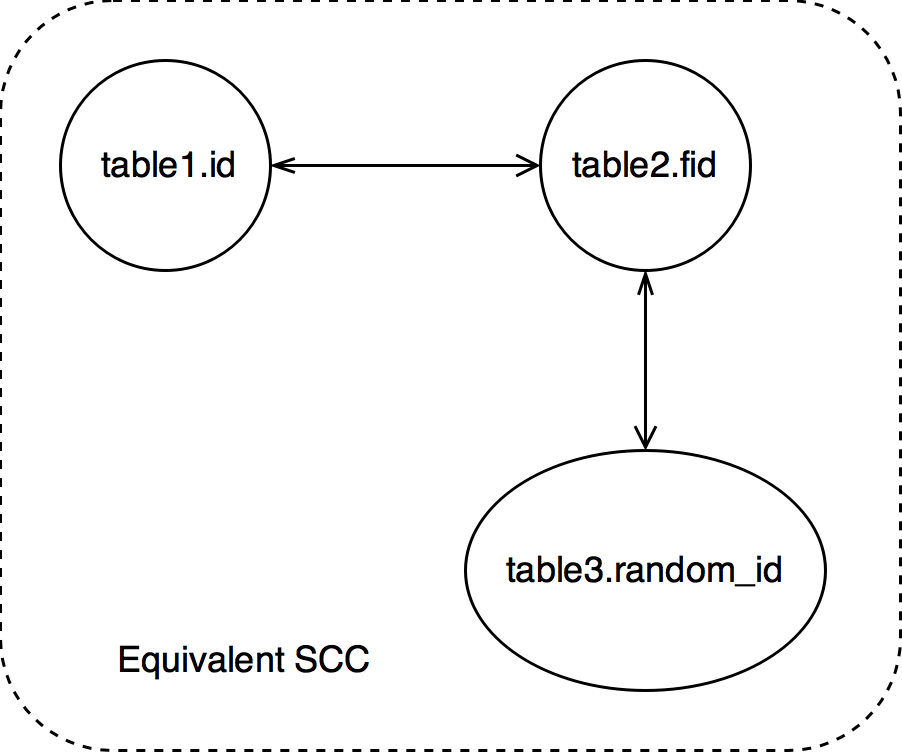
\includegraphics[height=4cm]{Chapters/5-Implementation/scc.png}}
\end{tabular}
\caption{Example of equivalence graph}
\end{figure}

To find the equivalences we traverse the join expression and look for qualified joins:
\begin{code}
\begin{minted}{ruby}
def find_equivalences(clause)
  if clause.is_a?(SQLParser::Statement::QualifiedJoin)
    [
      find_equivalences_search_condition(
        clause.search_condition.search_condition
      ),
      find_equivalences(clause.left),
      find_equivalences(clause.right),
    ].flatten
  elsif clause.is_a?(SQLParser::Statement::JoinedTable)
    [
      find_equivalences(clause.left),
      find_equivalences(clause.right),
    ].flatten
  else
    []
  end
end
\end{minted}
\caption{Traverse tree looking for qualified Join}
\label{fig:traversetreeequiv}
\end{code}

Once we find a qualified join we then look at the search condition for $=$ operations. A join expression can have multiple $=$ if they are joined by $\land$ so the library traverses all $\land$ nodes from the Boolean expression:
\begin{code}
\begin{minted}{ruby}
def find_equivalences_search_condition(search_condition)
  if search_condition.is_a?(SQLParser::Statement::And)
    [
      find_equivalences_search_condition(search_condition.left),
      find_equivalences_search_condition(search_condition.right),
    ].flatten
  elsif search_condition.is_a?(SQLParser::Statement::Equals)
    [
      {
        equivalence_left: search_condition.left,
        equivalence_right: search_condition.right,
      },
    ]
  else
    []
  end
end
\end{minted}
\caption{Looking for $=$ in search condition}
\label{fig:lookingequals}
\end{code}

To build the graph we use a Ruby library called RGL. RGL provides the implementation of various graph structures and graph algorithms (including the SCC algorithm). RGL does not support undirected graphs so we simply add two edges (from $v_1$ to $v_2$ and from $v_2$ to $v_1$). The process of building the graph is presented in listing \ref{fig:buildinggraph}.

\begin{code}
\begin{minted}{ruby}
def build_equivalence_graph
  graph = RGL::DirectedAdjacencyGraph.new

  join_conditions = @parsed_query.query_expression.table_expression.from_clause.tables.first

  equivalences = find_equivalences(join_conditions)

  equivalences.each do |equivalence|
    graph.add_edge(equivalence[:equivalence_left].to_sql, equivalence[:equivalence_right].to_sql)
    graph.add_edge(equivalence[:equivalence_right].to_sql, equivalence[:equivalence_left].to_sql)
  end

  graph.condensation_graph.vertices
end
\end{minted}
\caption{Building the equivalence SCC}
\label{fig:buildinggraph}
\end{code}

After the equivalence graph has been built, we check if there is an equivalent for every column.

\begin{code}
\begin{minted}{ruby}
equivalence = equivalences_list.detect do |equivalences|
  equivalences.include?(column.to_sql)
end

if equivalence.present?
  # transform qualified columns in sql form to two strings representing the
  # table and the column name
  table_name, column_name = equivalence.sort.first.remove("`").split(".")

  SQLParser::Statement::QualifiedColumn.new(
    SQLParser::Statement::Table.new(table_name),
    SQLParser::Statement::Column.new(column_name)
  )
else
  column
end
\end{minted}
\caption{Transforming equivalent columns}
\end{code}

\subsection{Transforming conditions from WHERE, HAVING, and JOIN conditions}
The WHERE and HAVING clauses and the JOIN condition are represented by a Boolean expression tree. When transforming these it is essential to ensure the structure of the expression is not altered - meaning that the before and after expressions are equivalent. To do this, the algorithm traverses the tree recursively.

\begin{code}
\begin{minted}{ruby}
def transform_tree(node)
  if node.is_a?(SQLParser::Statement::SearchCondition)
    node.class.new(
      transform_tree(node.left),
      transform_tree(node.right)
    )
  elsif node.is_a?(SQLParser::Statement::Between)
    transform_between(node)
  else
    node
  end
end
\end{minted}
\caption{Example of traversing a Boolean expression tree looking for \mintinline{mysql}{BETWEEN}}
\end{code}

\subsubsection{Transforming \mintinline{mysql}{BETWEEN} predicate}

A \mintinline{mysql}{column_name BETWEEN num1 AND num2} predicate will be transformed to two separate predicates: \mintinline{mysql}{column >= num1} and \mintinline{mysql}{column <= num2}. 

\begin{code}
\begin{minted}{ruby}
def transform_between(between)
  SQLParser::Statement::And.new(
    SQLParser::Statement::GreaterOrEquals.new(between.left, between.min),
    SQLParser::Statement::LessOrEquals.new(between.left, between.max)
  )
end
\end{minted}
\caption{Transforming a BETWEEN predicate}
\label{fig:transforming_a_betweeb}
\end{code}

\subsubsection{Transforming \mintinline{mysql}{NOT} comparison predicates}

In the case of \mintinline{mysql}{NOT} predicates, the transformation process simply transforms the predicate to its opposite:
\begin{enumerate}
    \item \mintinline{mysql}{>} becomes \mintinline{mysql}{<=}
    \item \mintinline{mysql}{>=} becomes \mintinline{mysql}{<}
    \item \mintinline{mysql}{<} becomes \mintinline{mysql}{>=}
    \item \mintinline{mysql}{>=} becomes \mintinline{mysql}{>}
\end{enumerate}

In addition to these 4 predicate types, \mintinline{mysql}{NOT} can also be used with other types of predicates which the library will not transform (e.g. \mintinline{mysql}{NOT LIKE} which cannot be easily transformed to remove the use of \mintinline{mysql}{NOT}).

\begin{code}
\begin{minted}{ruby}
def transform_not(not_statement)
  # Greater
  if not_statement.value.is_a?(SQLParser::Statement::Greater)
    SQLParser::Statement::LessOrEquals.new(not_statement.value.left, not_statement.value.right)
  elsif not_statement.value.is_a?(SQLParser::Statement::GreaterOrEquals)
    SQLParser::Statement::Less.new(not_statement.value.left, not_statement.value.right)
  # Less
  elsif not_statement.value.is_a?(SQLParser::Statement::Less)
    SQLParser::Statement::GreaterOrEquals.new(not_statement.value.left, not_statement.value.right)
  elsif not_statement.value.is_a?(SQLParser::Statement::LessOrEquals)
    SQLParser::Statement::Greater.new(not_statement.value.left, not_statement.value.right)
  else
    not_statement
  end
end
\end{minted}
\caption{Transforming NOT}
\label{fig:transforming_not}
\end{code}

\subsubsection{Transform \mintinline{mysql}{>} and \mintinline{mysql}{>=} to \mintinline{mysql}{<} and \mintinline{mysql}{<=}}

Transforming \mintinline{mysql}{>} and \mintinline{mysql}{>=} to \mintinline{mysql}{<} and \mintinline{mysql}{<=} is done by simply reverting the negating the condition.

\begin{code}
\begin{minted}{ruby}
def transform_comparison_predicate(predicate)
  if predicate.is_a?(SQLParser::Statement::Greater)
    SQLParser::Statement::Less.new(
      predicate.right,
      predicate.left
    )
  elsif predicate.is_a?(SQLParser::Statement::GreaterOrEquals)
    SQLParser::Statement::LessOrEquals.new(
      predicate.right,
      predicate.left
    )
  else
    predicate
  end
end
\end{minted}
\caption{Transforming \mintinline{mysql}{>} and \mintinline{mysql}{>=} to \mintinline{mysql}{<} and \mintinline{mysql}{<=}}
\label{fig:transforming_great}
\end{code}

\section{Library: extracting attributes from a canonicalized query}

While sql-parser provides the AST tree for the parsed query, it does not explicitly provide the components of a query. To extract them, the library makes use of the AST and makes various transformations in order to extract the components to a desired data structure. The resulting data structure might be similar to the AST (which is true for most components), but it might also be different (for instance the FROM expression is represented as a tree in the AST, but we can more clearly represent it as an array).

This extraction and transformation process helps in three important ways. First of all, it extracts the data in a format that can be easily compared by the grading algorithm. Second of all, equivalent types of components are extracted to a similar format (for instance the structure of the WHERE component is identical to the structure of the HAVING component). Lastly, the format can be defined in a way that is also easy to display on the front-end.

\subsection{Making defaults explicit}

Every \texttt{MySQL} query has certain default attributes. For instance, every \texttt{MySQL SELECT} query has a default uniqueness filter of \mintinline{mysql}{ALL}. This means that, while explicitly mentioning \mintinline{mysql}{ALL} will have no effect, it does not mean that it is making the query wrong. In order to accurately compare two queries, we must make the defaults explicit in both queries. The defaults will be made explicit during this extraction process.

\subsection{Format of components}

\begin{itemize}
    \item \textbf{Selected columns} are simply represented as an array of strings, where every string represents a selected column.
    \item \textbf{Order by} clause is represented as an array of hashes. Each hash has two attributes:
    \begin{enumerate}
        \item \mintinline{ruby}{column}: a string representing the full column name including the table name
        \item \mintinline{ruby}{position}: an integer representing the position in the order clause
    \end{enumerate}
    \item \textbf{Group} clause is represented as an array of strings, where every string represents a column.
    \item \textbf{Tables} clause is represented as an array of hashes.
    \begin{enumerate}
        \item The first element of the array is the base table (or sub-query) of the \mintinline{mysql}{FROM} clause. The item is represented as a hash containing the following keys:
        \begin{enumerate}
            \item \mintinline{ruby}{type}: either \mintinline{ruby}{"table"} or \mintinline{ruby}{"Subquery"}
            \item \mintinline{ruby}{table}: the table name or \mintinline{ruby}{attributes} in the case of sub-queries
            \item \mintinline{ruby}{sql}: the element represented as a SQL expression
        \end{enumerate}
        \item The other elements (the joined tables or joined sub-queries) of the array are represented as a hash containing the following keys:
        \begin{enumerate}
            \item \mintinline{ruby}{join_type}: the type of the join
            \item \mintinline{ruby}{table}: a hash that represents a table or sub-query. The format of the hash is the same one as the first element of the array.
            \item \mintinline{ruby}{searchcondition}: represents the join condition. Even if the search condition is similar to a Boolean component, at the moment, the join condition is represented simply as a string. The implication of this representation is that no partial grading is possible on the search condition.
            \item \mintinline{ruby}{sql}: the full SQL expression for the join (e.g. \mintinline{mysql}{LEFT JOIN table_name ON condition1 AND CONDITION 2})
        \end{enumerate}
    \end{enumerate}
    \item \textbf{Distinct filter} is represented as a simple string with a default value of \mintinline{mysql}{ALL}.
    \item \textbf{Limit} clause is represented as a hash with two keys: limit and offset. If the limit is not defined, then the value \texttt{inf} will be associated with it.
    \item \textbf{Where and Having} clauses are represented identically. There are two formats in which the library represents them as each format is used for a different purpose:
    \begin{enumerate}
        \item For the grading algorithm, these clauses are represented as binary trees.
        \item For the web application, these clauses are represented as trees (but not binary trees), where Boolean operators (e.g. \mintinline{mysql}{AND}) can have more than two children). For instance, the binary tree for expression ($ a \land b \land c$) has the following structure: 
        
\Tree[
    .$\land$
    [
        .$\land$
        [.$a$ ]
        [.$b$ ]
    ]
    [
        .$c$
    ]
]

while the tree format for the web application has the following structure:

\Tree[
    .$\land$
    [
        .$a$
    ]
    [
        .$b$
    ]
    [
        .$c$
    ]
]

This format allows the web application to display the clauses on the front-end in a format that is easier to understand.
    \end{enumerate}
\end{itemize}


\section{Library: partial grading}

In the design section of the algorithm (\ref{ch:des:grading}) we categorized the 8 components of a \mintinline{mysql}{SELECT} query into 3 types of components: simple, array, and Boolean. This section will not present the full implementation of the grading algorithm, as the algorithm has already been explained. For the full code, please refer to the source code under the folder \texttt{lib/sql\_assess/grader/base.rb}.

Implementing the algorithm was straightforward once the design of the algorithm has been finalized. In general, the algorithm makes use of only basic iterations and if statements.

\subsection{Grading simple components}
As mentioned in the design section (\ref{ch:des:grading}), grading simple components is done by comparing the attributes of the two hashes with a finite amount of keys. In these cases (limit clause and distinct filter), the grade is simply calculated by looking at the two extracted components.

\begin{code}
\begin{minted}{ruby}
def grade
  if @student_distinct == @instructor_distinct
    1.0
  elsif @student_distinct == 'DISTINCT' && @instructor_distinct == 'DISTINCTROW'
    0.5
  elsif @student_distinct == 'DISTINCTROW' && @instructor_distinct == 'DISTINCT'
    0.5
  else
    0
  end
end
\end{minted}
\caption{Partial grading of distinct filter}
\end{code}

\subsection{Grading array components}

In the case of array components, graders just need to implement a \mintinline{ruby}{match_score}, as the \mintinline{ruby}{Grader::Base} class already implements the algorithm described in section \ref{ch:des:grading}. As previously mentioned, the code for the array grading is included in the Appendix under the source code for file \texttt{lib/sql\_assess/graders/base.rb}.

\begin{code}
\begin{minted}{ruby}
def match_score(column1, column2)
  if column1 == column2
    2
  else
    table_name1, column_name1 = column1.split('.')
    table_name2, column_name2 = column2.split('.')

    if table_name1 == table_name2
      2.0 / levenshtein_distance(column_name1, column_name2)
    else
      0
    end
  end
end
\end{minted}

\caption{Match score for columns}
\end{code}

\subsection{Grading Boolean components}

Grading Boolean components requires the implementation of two methods:
\begin{enumerate}
    \item A method that extracts the leaves of the tree:
    \begin{code}
    \begin{minted}{ruby}
def get_leaves(node)
  if node.nil?
    nil
  elsif node[:is_inner] == false
    node
  else
    [
      get_leaves(node[:left_clause]),
      get_leaves(node[:right_clause]),
    ].flatten
  end
end
    \end{minted}
    \caption{Extracting the leaves of the tree}
    \end{code}
    \item A method that implements the grading of the tree. The algorithm was already described in the design section. For the full code, please refer to \texttt{lib/sql\_assess/grader/where.rb} 
\end{enumerate}

\section{Library: providing hints}

Currently, the hints provided are only at the component level. Every wrong component has a possible hint if the match score is not 100\%. The library will check all components where the match score is not 100\% and select the most relevant hint. The relevance of the hint is predefined in the algorithm based on the component type.

\begin{tabularx}{\textwidth}{|l|X|X|}
\hline
\textbf{Importance} & \textbf{Component} &
\textbf{Hint message}\\\hline
\endhead
1 & Tables & Are you sure you are selecting the right tables? \\\hline
2 & Columns & Check what columns you are selecting. \\\hline
3 & Group & Are you grouping by the correct columns? \\\hline
4 & Where & Looks like you are selecting the right columns, but you are not selecting only the correct rows. \\\hline
5 & Having & Looks like you are selecting the right columns, but you are not selecting the correct rows. \\\hline
6 & Distinct filter & What about duplicates? What does the exercise say? \\\hline
7 & Limit & Are you selecting the correct number of rows? \\\hline
8 & Order by & Are you ordering the rows correctly? \\\hline

\end{tabularx}

\section{Web application: user management}
\subsection{Authentication}
Authentication in the web application is implemented using the devise library. Devise is the most popular authentication library built for Ruby on Rails with over 18000 stars on GitHub and over 33 million downloads on Ruby gems. In addition to a simple log-in / log-out functionality, devise provides many out-of-the-box features: recovering password, sending and handling confirmation emails, integration with OAuth providers such as Facebook login, etc. An important aspect of any authentication system is how passwords are stored in the database. Devise uses the bcrypt algorithm to hash passwords. bcrypt is a password hashing function \citep{wiki:bcrypt} used in OpenBSD and Suse Linux and trusted by many big companies such as Dropbox \citep{dropbox:authentication},

\subsection{Authorization}
To handle roles, the application uses two tools: a role field on the user database, and the pundit library. pundit is a library that provides ''authorization through Object Oriented Design and pure Ruby classes'' \citep{github:pundit}. Every user has a role that is either student or admin.

Pundit makes use of the concept of policies, which describe the authorization rules for a model. This means that every model will have an associated policy. A policy has the following attributes:

\begin{itemize}
    \item A policy is instantiated in the controller with the current user and, optionally, with an instance of an object.
    \item The pundit policy files define methods whose naming convention follows the Ruby on Rails controller action names described in section: \ref{ch:design:web:controller}. This means that a policy defines the following methods: \mintinline{ruby}{def index?}, \mintinline{ruby}{def show?}, \mintinline{ruby}{def create?}, \mintinline{ruby}{def new?}, \mintinline{ruby}{def update?}, \mintinline{ruby}{def edit?}, \mintinline{ruby}{def destroy?}. The method returns whether the user has access to perform the action on a certain object or class. An example of this can be seen in listing \ref{fig:policy_challenge}, which makes it clear that only admins can create new challenges.

\begin{code}
\begin{minted}{ruby}
class ChallengePolicy < ApplicationPolicy
  # ...
  def create?
    user.admin?
  end
  # ...
end
\end{minted}
\caption{Example policy for Challenge creation}
\label{fig:policy_challenge}
\end{code}
    \item The pundit method provides the \mintinline{ruby}{authorize} method to a Ruby on Rails controllers that automatically instantiates a policy, and automatically calls the correct method. An example of the usage of the authorize method is seen in listing \ref{fig:policy_challenge_usage} where the authorize method is called to ensure that the user has access to the challenge. If the user is not authorized, then a response with HTTP code 401 (Unauthorized) is returned to the user.
\begin{code}
\begin{minted}{ruby}
def show
  @challenge = Challenge.find_by!(id: params.require(:id))
  authorize @challenge
  # ...
end
\end{minted}
\caption{Example of policy usage}
\label{fig:policy_challenge_usage}
\end{code}
\end{itemize}

\section{Web application: front-end implementation}
Although not too much time has been spent on the web application's front-end, the way it has been built tried to take into consideration future work that might occur on it. 

Therefore, the web application front-end is built using a modern architecture. While pages used to be generally powered by HTML and CSS only, nowadays JavaScript (JS) is almost always used in all applications. However, JS in large applications is no longer used just by including a file in HTML's \mintinline{html}{<head>}. The increased popularity of JS frameworks (React, Angular, Vue, etc.) meant that most JS apps now use a build system. To prepare for this, the web application uses Webpack.  Webpack is the  module bundler endorsed by both React and Vue.

In addition to just bundling JS, Webpack also bundles other types of files. One important type of file bundled is represented by SCSS files which are used in the web application. SCSS is, according to their creators, ''CSS with superpowers'' \citep{SassSynt0:online}. SCSS provides many additional features such as functions that allow us to create styles faster. For instance, the CSS styles used for displaying the \mintinline{mysql}{WHERE} clause as a tree with 10 levels can be easily defined in just a few lines of code using functions (which do not exist in vanilla CSS), instead of defining a style for each level.

%TC:ignore
\begin{code}
\begin{minted}{scss}
@for $i from 0 through 10 {
  .where-clause-depth-#{$i}::before {
    content: repeat('··', $i + 1);
    margin-right: 4px;
    color: grey;
  }
}
\end{minted}
\caption{Defining tree representation of WHERE}
\label{fig:scss}
\end{code}
%TC:endignore

The front-end design is currently built using three tools:
\begin{enumerate}
    \item Bootstrap: an open-source front-end framework that provides CSS and JS for most common web page components.
    \item codemirror: a basic code editor that can be included in an HTML page. An example of codemirror is presented in figure \ref{fig:codemirror}.
\begin{figure}[H]
    \centering
    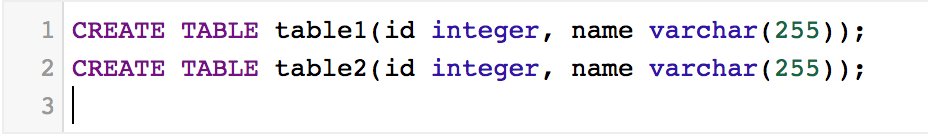
\includegraphics[width=\textwidth]{Chapters/5-Implementation/codemirror.png}
    \caption{Example of codemirror}
    \label{fig:codemirror}
\end{figure}
    \item  highlight.js: a basic code highlighter (for static fields) that can be included in a HTML page. An example of highlight.js is presented in figure \ref{fig:highlightjs}.
\begin{figure}[H]
    \centering
    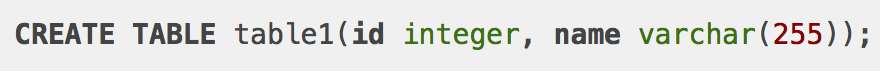
\includegraphics[width=\textwidth]{Chapters/5-Implementation/higlightjs.png}
    \caption{Example of highlight.js}
    \label{fig:highlightjs}
\end{figure}
\end{enumerate}

\section{Web application: instructor's view}

\begin{figure}[H]
    \centering
    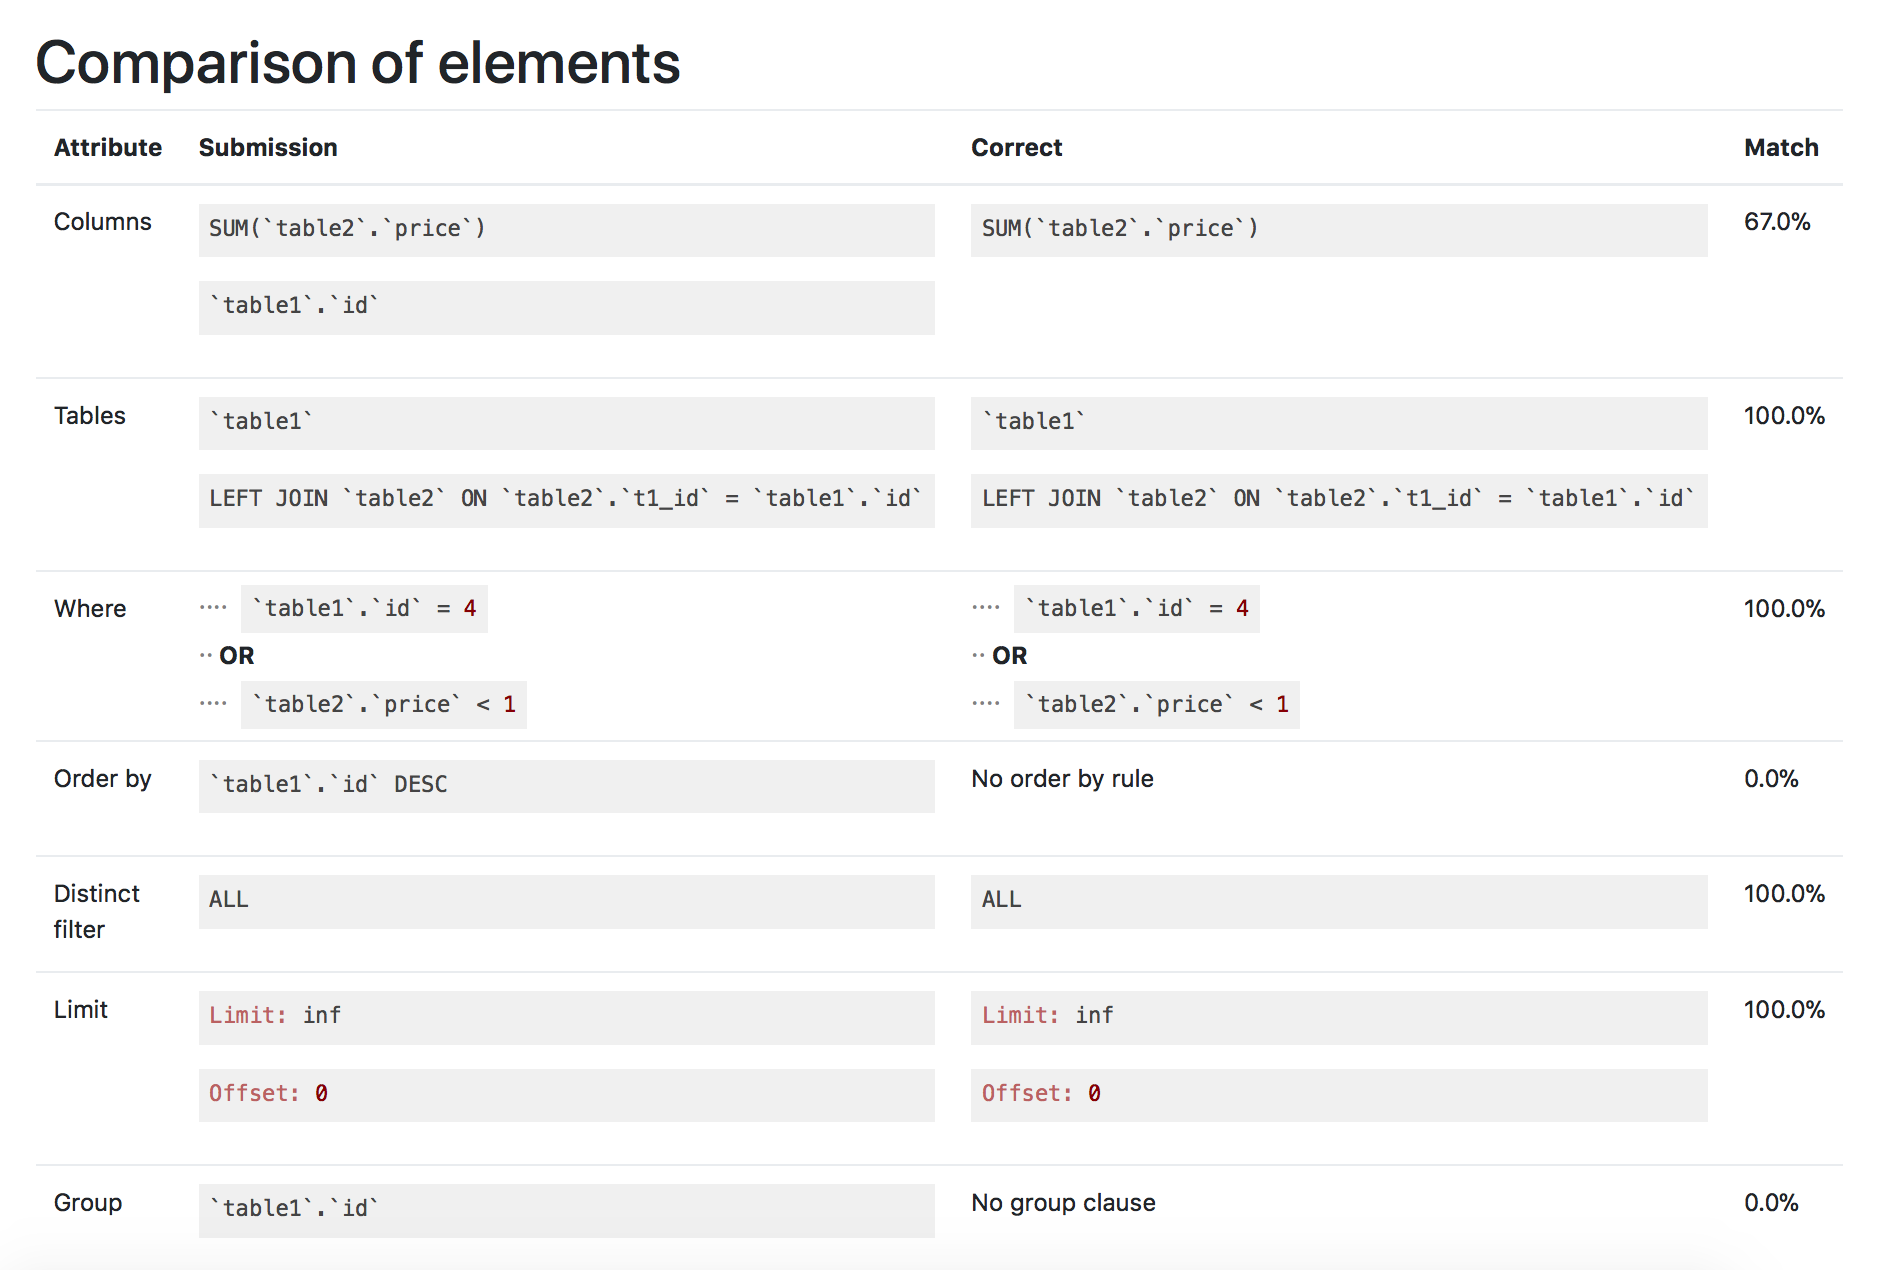
\includegraphics[width=\textwidth]{Chapters/4-Design/components.png}
    \caption{Instructor's view of a submissions}
    \label{fig:instructors_view}
\end{figure}

Compared to students, instructors can view a detailed breakdown of any submissions (presented in figure \ref{fig:instructors_view}). In this view they can see the canonicalized components of each query, and what grade score has been given to each component. The web application simply displays the information received from the library after the submission has been assessed.

In addition to viewing individual submissions, instructors can also download a CSV file containing the best result for each student for a challenge. The code for obtaining the best grade is included in listing \ref{fig:gettingbestgrade}. The CSV file is the generated by the \mintinline{ruby}{SubmissionsController} using the Ruby library csv. The code for generating the CSV is presented in listing \ref{fig:generatingcsv}.

\begin{code}
\begin{minted}{ruby}
class Challenge
  # ..
  has_many :submissions
  # ..
  def best_submissions
    submissions.select('max(grade) as max_grade, user_id').group(:user_id)
  end
  # ..
end
\end{minted}
\caption{Getting the best grade for a challenge}
\label{fig:gettingbestgrade}
\end{code}


\begin{code}
\begin{minted}{ruby}
format.csv do
  submissions = @challenge.best_submissions.includes(:user)

  authorize submissions

  final_csv = CSV.generate do |csv|
    csv << %w[email grade]

    submissions.each do |submission|
      csv << [submission.user.email, submission.max_grade]
    end
  end

  send_data(
    final_csv,
    filename: "grades_for_#{@challenge.title}.csv",
    type: :csv
  )
end
\end{minted}
\caption{Generating CSV}
\label{fig:generatingcsv}
\end{code}

\section{Testing}
Testing any software is an essential step in the development process. The purpose of software testing is to validate that the software is behaving as intended \citep{lit:software_testing}. Testing can also be used to check if the requirements have been correctly implemented. As previously mentioned in the development process section (\ref{ch:reqandspec:sec:spec:subsec:dev_process}), testing has been an integral part of the project, with new tests written for all new features added.

Testing is especially important in dynamic languages like Ruby, due to the lack of types and a compile step. Ruby uses what is sometimes called \textit{duck typing} which is enforced using the duck test: ''If it walks like a duck and it quacks like a duck, then it must be a duck.'' \citep{wiki:duck_typing}. That means that Ruby only cares if an object implements a method, it does not care about the type of the object on which the method is called. While this might help developers move faster, duck typing can lead to an increased amount of errors as no type checking is done until run-time. In addition, without a proper test suite, re-factoring can become a nightmare for someone working in Ruby, as they have no confidence the changes they are making will not affect the existing ones.

To ensure the software is working according to the requirements and that future re-factors will be made easily, the project uses two types of testing: unit testing and integration testing.

\subsection{Unit testing}

Unit testing refers to the testing of individual units of code or groups of related units \citep{unit_testing}. The purpose of unit testing is to make sure the code meets the specifications \citep{Olan2003}. In order to unit test the two parts of the application, we are using RSpec, which is a DSL testing tool for Ruby \citep{wiki:rspec}. Overall, the library and the web application have in total over 300 unit tests.

In Ruby and RSpec, tests for a class go in an associated \texttt{class\_name\_spec.rb} located in the \texttt{spec/} folder. RSpec's DSL provides multiple methods that allow most unit tests to be easily to read and understood, as the resulting format of unit tests is similar to an English sentence.

\begin{code}
\begin{minted}{ruby}
context "when there is *" do
  it "returns the query containing all columns in select" do
    expect(subject.transform("SELECT * FROM table1"))
      .to eq("SELECT `table1`.`id1`, `table1`.`id2` FROM `table1`")
  end
end
\end{minted}
\caption{Example of unit test for \mintinline{mysql}{*} transform}
\label{fig:example_unit_test}
\end{code}

Both the application and the library have unit tests covering 100\% of the code. This means that every unit of code is executed at least once during the test suite. However, no test suite can ensure that bugs are not presented even if it has 100\% test coverage. It is worth mentioning that the utility of code coverage is highly debated. Work done by \cite{msft_testing} at Microsoft Research showed that more test coverage does not necessarily result in fewer bugs. This can be associated with many factors such as the increased difficulty in testing complex code. More important is the fact that code coverage is not correlated with how users are using the app: if users spent most time using features that represent 1\% of the code, testing that 1\% is more important that achieving a high code coverage in the rest of the application. \cite{msft_testing} suggests that it is more important to have better test coverage in the more complex part of the application.

To avoid the issues described by \cite{msft_testing}, both test suites try to include more tests for sensitive parts of the applications (such as canonicalization and grading process), with less tests covering non-core functionality.

\subsection{Integration testing}

A more important type of testing is integration testing. Integration testing refers to the testing of the interaction between multiple units of the application. Integration testing makes sure that all units of an application work together according to the requirements.

\subsubsection{Integration testing in the web application}

Integration testing in a web application has the role of checking if all MVC components integrate correctly. Integration testing was done using RSpec and Capybara. Capybara is a tool that simulates scenarios by directly controlling a web browser driver. This means that Capybara takes a set of instructions (such as click this button, type in this field, etc.) and executes them on an actual browser. Integration testing with Capybara follows a very similar pattern to user stories. In fact, all user stories for a web application can be implemented as Capybara tests.

\begin{code}
\begin{minted}{ruby}
context "logged in as an admin" do
  context "with correct queries" do
    it "creates the challenge and displays the query" do
      visit "/challenges/new"

      fill_in "Title", with: "Challenge 1"
      fill_in "Content", with: "Challenge 1 content"
      fill_in "Sql schema", with: "CREATE TABLE t1(id integer);"
      fill_in "Sql seed", with: "INSERT INTO t1(id) VALUES (1), (2);"
      fill_in "Sql correct query", with: "SELECT * FROM t1"

      click_button "Create"

      expect(page).to have_text("Successfully created")

      expect(page).to have_text("CREATE TABLE t1(id integer);")
      expect(page).to have_text("INSERT INTO t1(id) VALUES (1), (2);")
      expect(page).to have_text("SELECT * FROM t1")
    end
  end
end
\end{minted}
\caption{Example of integration test using Capybara.}
\end{code}

\subsubsection{Integration testing in the library} \label{ch:impl:sec:testing:subsec:integ_library}

Integration testing in the library is the testing of the \mintinline{ruby}{Assesor} class which internally uses all other classes. Testing the assessor is equivalent with testing the integration between the database connection and secure querying, the canonicalization process, the extraction of components, and finally the grading process. In addition to the integration tests for the assessor, other integration tests are represented by the tests for \mintinline{ruby}{QueryTransformer}, which uses all transformations to transform a query.

Integration tests are defined in a \texttt{.yml} file that is then loaded, and then tests are created based on that file. Listing \ref{fig:dynamically_testing} shows how integration tests for the transformer are automatically defined from a file.

\begin{code}
\begin{minted}{ruby}
yaml = YAML.load_file("spec/fixtures/transformer_integration_tests.yml")
yaml.each do |test|
  it "transforms #{test['query']} to #{test['expected_result']}" do
    # Seed data
    connection.multiple_query(test["schema"])
    # Check if queries from file are correct
    connection.query(test["query"])
    connection.query(test["expected_result"])
    # Check transformation
    expect(subject.transform(test["query"])).to eq(test["expected_result"])
  end
end
\end{minted}
\caption{Dynamically defining tests based on a file}
\label{fig:dynamically_testing}
\end{code}